\section{Methods}
\label{sec:methods}

In this section, we describe the methodology we use to solve the ride-sharing problem. First, we state the problem, then briefly introduce the pipeline, followed by a detailed discussion of each step. As discussed before, a multi-driver ride-sharing problem is computationally difficult to solve in a reasonable runtime. Due to this, we introduce a decomposed, three-step approach rather than trying to formulate the problem as a single integer linear program.

\subsection{Problem formulation}

Let $\mathcal{N}$ be the set of customers and $\mathcal{K}$ the set of drivers. Each customer $i$ has a set $\mathcal{P}_i\subset\mathcal{K}$ of driver preferences. Customer $i$ can be assigned to driver $k$ only if $ k$ is in customer $ i$'s preference set. This relationship between customers and drivers can be modelled using a graph.

\begin{definition}[Graph]
A \emph{graph} $G = (V, E)$ consists of a finite set $V$ of \emph{vertices} and a set $E$ of \emph{edges}, where each edge $\{u, v\} \in E$ joins two distinct vertices $u, v \in V$. Each edge also carries a number $w(e)$, making the graph a \emph{weighted graph}.
\end{definition}

The sets $\mathcal{N}$ and $\mathcal{K}$ form two disjoint sets of vertices. These sets can be connected uniquely by connecting each vertex $i\in\mathcal{N}$ to all vertices in $\mathcal{P}_i$. Since $\mathcal{P_i}\subset\mathcal{K}$, a vertex $i\in\mathcal{N}$ can be connected only to a vertex $k\in\mathcal{K}$, making the graph bipartite. 

\begin{definition}[Bipartite graph]
A graph is \emph{bipartite} if its vertex set can be partitioned into two disjoint sets $V = A \cup B$ such that every edge joins a vertex in $A$ to a vertex in $B$.
\end{definition}

Each customer $i$ has a wanted pickup time $U_i$ and a ride duration $R_i$, and each driver $k$ works within a shift window $[S_k, H_k]$, meaning the driver is available from time $S_k$ until time $H_k$. 

The objective is to calculate optimal schedules for each driver to minimise the number of unserved customers, customer pickup delays, and driver idle time. This means finding a suitable set of customers for each driver. We define the problem as a combination of matching and optimisation. 

\begin{definition}[Matching]
A \emph{matching} in a graph is a set of edges of which no two share a vertex. We use a capacitated generalization in which each vertex $v$ may be connected by at most $c(v)$ chosen edges, where $c(v)$ is a per-vertex capacity.
\end{definition}

The idea is to first find, for each driver $k$, an assignable set $A_k \subseteq \mathcal{N}$ of customers by computing a matching on the preference graph. Then, using the assignable sets, we optimize an initial schedule for each driver with integer linear programming (ILP). Because drivers are scheduled independently, a single customer can be assigned to several drivers, causing conflicts. To resolve the conflicts, we perform a conflict-resolution step and iterate the scheduling to improve the total objective value. As a result, we have three separate problems to define and solve.

These three subproblems, matching, scheduling and conflict resolution, together form a pipeline that finds a solution to the whole scheduling problem. It takes the bipartite graph of preferences as input and produces optimised schedules and a set of metrics as output. Figure~\ref{fig:pipeline} shows the pipeline overview.

\begin{figure}[H]
  \centering
  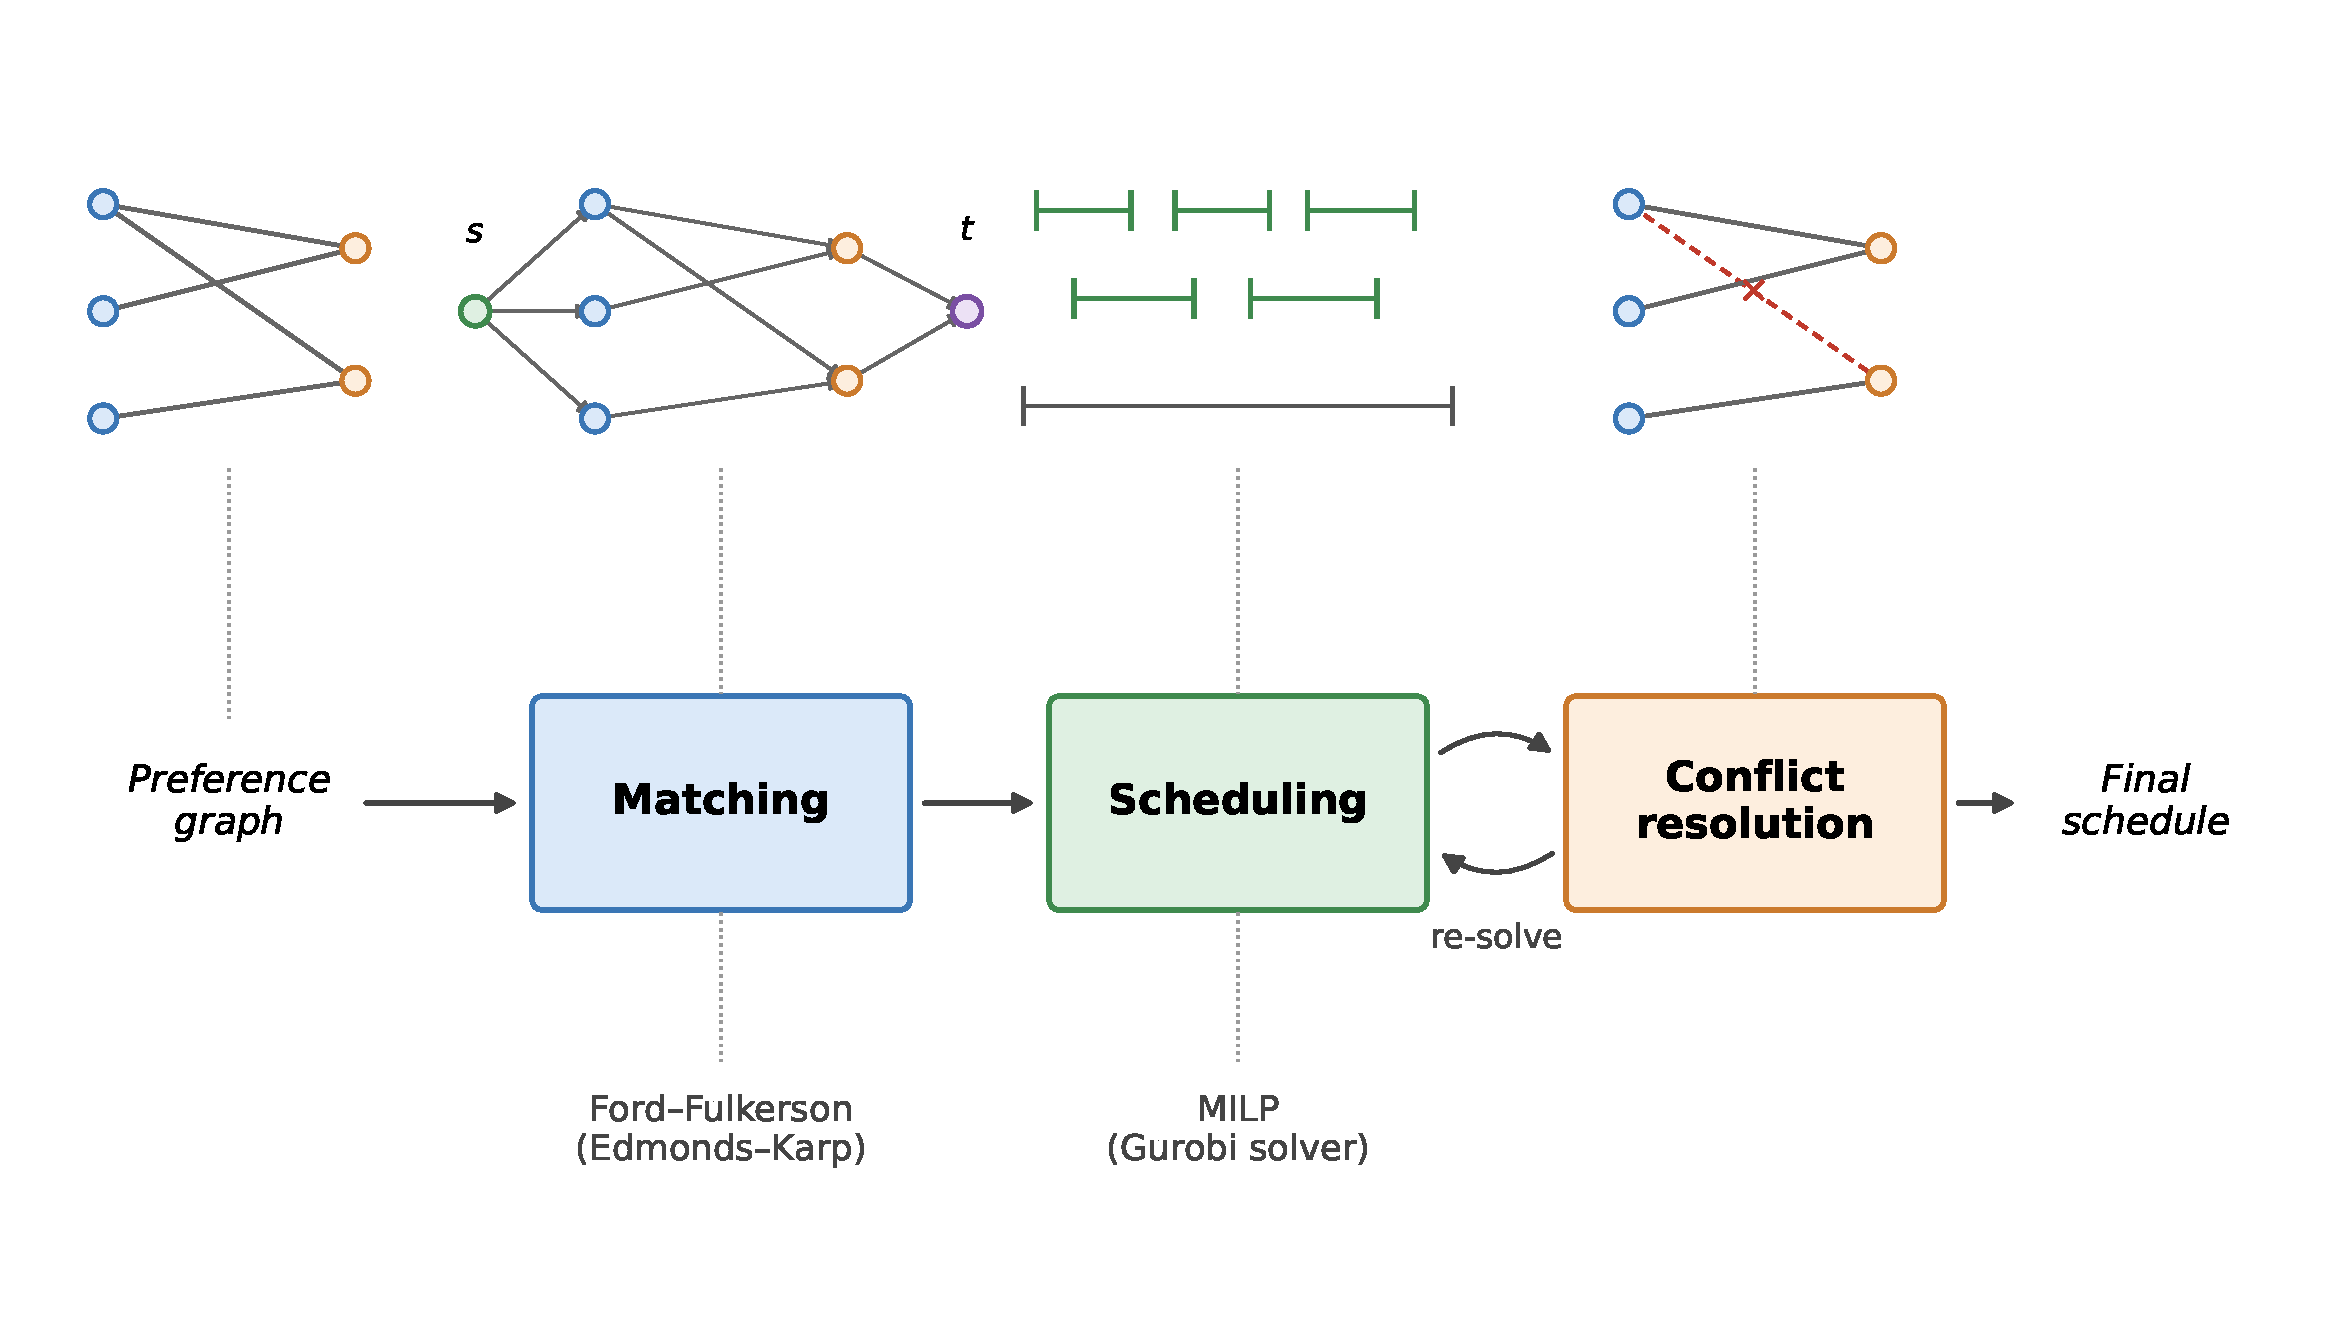
\includegraphics[width=1.05\textwidth]{figures/pipeline_process_flow.pdf}
  \caption{The outline of the scheduling pipeline}
  \label{fig:pipeline}
\end{figure}

\subsection{Matching via maximum flow}

The first subproblem in the scheduling pipeline is matching. Each customer $i$ provides a set of driver preferences $\mathcal{P}_i$, and the number of drivers a customer can be matched to is capped. A driver can be matched to as many customers as possible. The matching subproblem provides the assignable sets $A_k$ for each driver $k$ as output. We formulate the subproblem as a capacitated bipartite matching problem.

\begin{problem}[Matching customers to drivers]
\label{prob:matching}
Let $G = (\mathcal{N} \cup \mathcal{K}, E)$ be the bipartite preference graph with an edge set 
\[
E = \bigl\{\, \{i, k\} : i \in \mathcal{N},\ k \in \mathcal{P}_i \,\bigr\}
\]
and let $w(i) \in \mathbb{Z}$ be the weight of customer $i$, that is, the maximum number of drivers customer $i$ may be matched to and let $w(k) \in \mathbb{Z}$ be the weight of driver $k$, that is, the maximum number of customers driver $k$ may serve.\\
Find a matching $M \subseteq E$ of maximum cardinality that respects the weights, i.e. solve
\begin{align}
  \max_{M \subseteq E} \quad & |M| \label{eq:matching-obj}\\
  \text{s.t.} \quad
  & \bigl|\{\, k : \{i,k\} \in M \,\}\bigr| \le c(i) && \text{for all } i \in \mathcal{N}, \label{eq:matching-cust}\\
  & \bigl|\{\, i : \{i,k\} \in M \,\}\bigr| \le c(k) && \text{for all } k \in \mathcal{K}. \label{eq:matching-drv}
\end{align}
The matching $M$ defines an assignable set for each driver $k$
\[
A_k = \bigl\{\, i \in \mathcal{N} : \{i, k\} \in M \,\bigr\}.
\]
\end{problem}

We solve Problem~\ref{prob:matching} using maximum flow with the Ford––Fulkerson algorithm~\citep{ford1957simple}. The Ford–Fulkerson algorithm computes the maximum flow in a directed graph. Ford–Fulkerson constructs a copy of the original graph, called the residual graph, and uses it to compute the maximum flow by repeatedly finding augmenting paths. An augmenting path is a path through the graph with remaining capacity. We use a variant of the Ford–Fulkerson algorithm called the Edmonds–Karp algorithm~\citep{edmonds1972theoretical}, which computes augmenting paths using breadth-first search. Algorithm~\ref{alg:ff} provides the algorithm pseudocode. We record the wall-clock time for the matching process so we can report the Ford–Fulkerson runtime alongside the solution.

\begin{algorithm}[H]
\caption{Ford–Fulkerson with breadth-first search (Edmonds–Karp)}
\label{alg:ff}
\begin{algorithmic}[1]
\Require directed graph $G = (V, E)$ with capacities $w$, source $s$, sink $t$
\Ensure the maximum flow value $f$
\ForAll{$(u, v) \in E$} \Comment{initialize the residual capacities}
  \State $r(u, v) \gets w(u, v)$
  \State $r(v, u) \gets 0$
\EndFor
\State $f \gets 0$
\Loop
  \State find a shortest path $p$ from $s$ to $t$ using breadth-first search over the edges with $r(u, v) > 0$
  \If{no such path exists}
    \State \Return $f$
  \EndIf
  \State $b \gets \min_{(u, v) \in p} r(u, v)$ \Comment{bottleneck of the path}
  \ForAll{$(u, v) \in p$} \Comment{push $b$ units of flow along $p$}
    \State $r(u, v) \gets r(u, v) - b$
    \State $r(v, u) \gets r(v, u) + b$
  \EndFor
  \State $f \gets f + b$
\EndLoop
\end{algorithmic}
\end{algorithm}

To compute the maximum flow, the Ford–Fulkerson algorithm needs a single source, a vertex where all flow is created, and a single sink, a vertex where all flow is consumed. We add these vertices so the source connects to every customer vertex and the sink to every driver vertex. The weights of the outgoing edges from a source set how many drivers a customer may choose from, and the weights of the incoming edges to a sink set a driver's capacity. Figure~\ref{fig:bipartite} shows the resulting
bipartite structure with the added source and sink.

\begin{figure}[H]
  \centering
  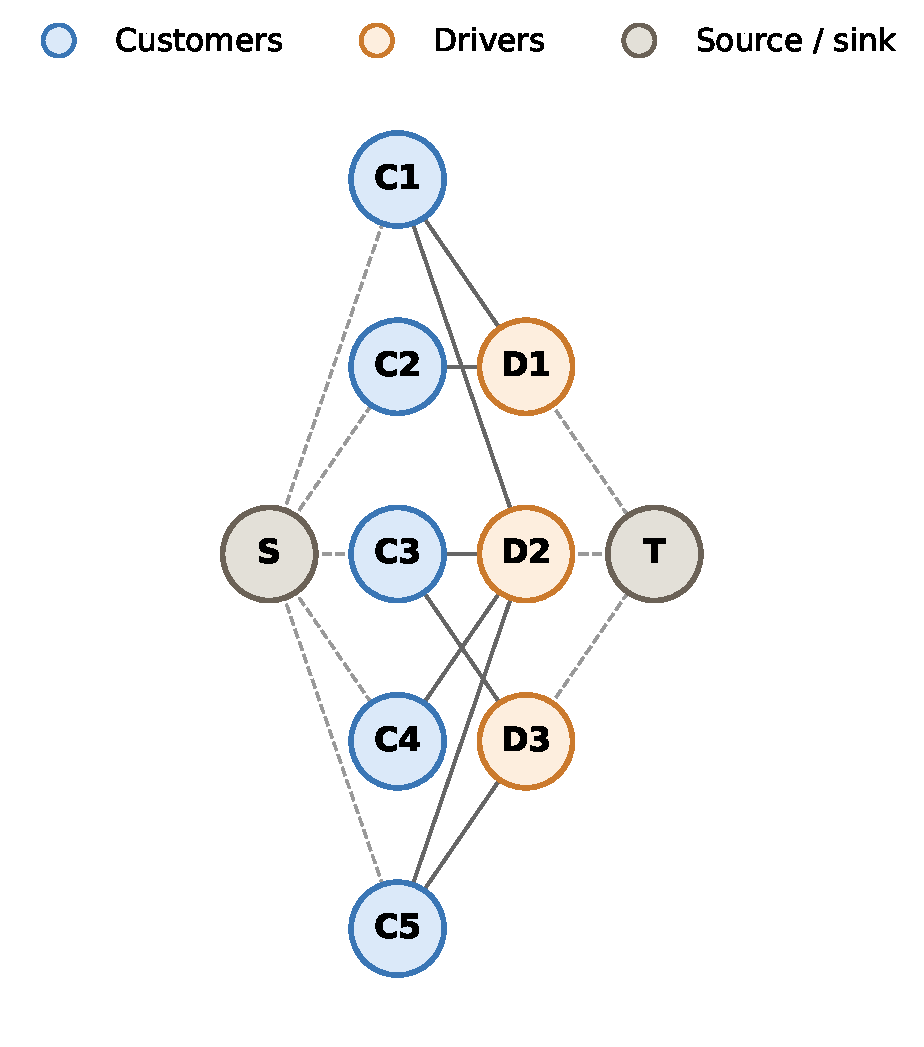
\includegraphics[height=0.6\textheight]{figures/bipartite_graph.pdf}
  \caption{A bipartite customer-driver graph with the source and sink.}
  \label{fig:bipartite}
\end{figure}

The customer-driver matching is read from the residual graph. For every edge $(c, d)$ between a customer $c$ and a driver $d$ in the original graph, the flow used along that edge equals the original capacity minus the remaining residual capacity. If this used flow is strictly positive, we record $(c, d)$ as a matched pair. From these matched pairs, we construct the sets of assignable customers. We record the average number of customers per driver, drivers per customer and also the coverage percentage, that is, the share of customers that were matched to at least one driver.

\subsection{Per-driver scheduling ILP}

After the matching step, we solve each driver's schedule separately using integer linear programming. The matching subproblem provides, for each driver $k$, the set $A_k$ of customers that $k$ is allowed to serve. This subproblem provides the initial schedules of each driver $k$ as output. A customer may be assigned to multiple drivers as the drivers are scheduled independently.

\begin{problem}[Scheduling customers for a driver]
\label{prob:scheduling}
Let $k$ be a driver with a shift window $[S_k, H_k]$ and an assignable set $A_k$ and let each customer $i \in A_k$ have a wanted pickup time $U_i$ and a ride duration $R_i$. Find a set $C_k \subseteq A_k$ of served customers and a pickup time $t_i$ for each $i \in C_k$ such that
\begin{enumerate}
  \item each ride lies within the shift and its pickup delay is bounded: $\max(U_i, S_k) \le t_i \le U_i + E_{\max}$ and $t_i + R_i \le H_k$,
  \item the rides of driver $k$ do not overlap, and the break between two consecutive rides is at least $B_{\min}$ and at most $B_{\max}$ minutes,
  \item the last ride ends within $B_{\max}$ minutes of the shift end $H_k$,
\end{enumerate}
minimizing the weighted sum
\[
D \sum_{i \in C_k} (t_i - U_i)
+ P\,\bigl|A_k \setminus C_k\bigr|
+ I \Bigl( (H_k - S_k) - \sum_{i \in C_k} R_i \Bigr)
\]
of the total pickup delay, the number of unserved customers, and the driver's idle time, with given weights $D$, $P$, and $I$.
\end{problem}

We solve Problem~\ref{prob:scheduling} with an independent time-indexed ILP for each driver $k$. We discretise time into slots of width $\Delta t$, one minute by default. For every customer $i \in A_k$ and every feasible start slot $t$, we introduce a binary variable $x_{i,t} \in \{0, 1\}$ that equals one if and only if customer $i$'s ride starts at slot $t$ on driver $k$. A start slot $t$ is feasible if and only if

\begin{align}
t \cdot \Delta t        &\geq \max(U_i, S_k), \label{eq:feas-start} \\
t \cdot \Delta t + R_i  &\leq H_k, \label{eq:feas-end} \\
t \cdot \Delta t - U_i  &\leq E_{\max}. \label{eq:feas-delay}
\end{align}

Constraint~\eqref{eq:feas-start} schedules the customer's pickup after both their wanted pickup time and the driver's shift start, \eqref{eq:feas-end} ensures the ride ends before the end of the driver's shift, and \eqref{eq:feas-delay} caps the pickup delay at $E_{\max}$. Let $T_i$ denote the set of feasible start slots for customer $i$ on driver $k$ and let $e_{i,t} = t \cdot \Delta t + R_i$ be the end of ride $(i,t)$. Let $N_{i,t} = \{(j, t') : j \in A_k \setminus \{i\},\ t' \in T_j, e_{i,t} < t' \cdot \Delta t \leq e_{i,t} + B_{\max}\}$ be the rides that could follow $(i,t)$, that is, those starting within $B_{\max}$ minutes of its end. Let $r_i = \lceil R_i / \Delta t \rceil$ be the number of slots a ride covers. To enforce a minimum break of $B_{\min}$ minutes between consecutive rides, inflate each ride's time footprint from $r_i$ to $r_i + b$, where $b = \lceil B_{\min} / \Delta t \rceil$. The ILP is

\begin{align}
\min \quad & D \sum_{i \in A_k} \sum_{t \in T_i} (t \cdot \Delta t - U_i) x_{i,t} \\
    +\quad & P \sum_{i \in A_k} ( 1 - \sum_{t \in T_i} x_{i,t} ) \\
    +\quad & I ( (H_k - S_k) - \sum_{i \in A_k} \sum_{t \in T_i} R_i x_{i,t} ) \label{eq:obj} \\
\text{s.t.} \quad 
\sum_{t \in T_i} x_{i,t} &\leq 1, && \forall i \in A_k, \label{eq:assign} \\
\sum_{\substack{i \in A_k, \, t \in T_i \\ t \leq \tau < t + r_i + b}} x_{i,t} &\leq 1, && \forall \text{ slot } \tau, \label{eq:overlap} \\
x_{i,t} &\leq \sum_{(j,t') \in N_{i,t}} x_{j,t'}, && \forall (i,t) \text{ s.t. } e_{i,t} + B_{\max} < H_k, \label{eq:succ} \\
& x_{i,t} \in \{0, 1\}, && \forall i \in A_k, \, t \in T_i. \label{eq:integrality}
\end{align}

The objective~\eqref{eq:obj} has three terms. The first minimizes total pickup delay, weighted by $D$. The second penalises each unserved customer by $P$. The third term, weighted by $I$, penalises the driver's idle time over the shift. Constraint~\eqref{eq:assign} serves each customer at most once, and \eqref{eq:overlap} forbids overlapping rides on the same driver by allowing at most one active ride in any slot $\tau$. Constraint~\eqref{eq:succ} bounds the breaks between rides to a maximum of $B_{\max}$ by requiring each ride to have a successor during the subsequent $B_{\max}$ minutes if there are more than $B_{\max}$ minutes of the driver's shift left after the drop-off of that ride. 

We use Gurobi (\citep{gurobi}) to optimize the ILPs. As the ILPs are independent of each other, we utilize parallelization to solve them in a less amount of time. From the solution, for each assigned customer $i$, we read their chosen start slot and realised pickup delay $\max(0,\, t \cdot \Delta t - U_i)$.

\subsection{Conflict resolution between drivers}

Since we scheduled each driver independently in the scheduling subproblem, the same customer can be assigned to more than one driver. Thus, we need to resolve conflicts between drivers so that each customer is served by at most one driver.

\begin{problem}[Conflict resolution]
\label{prob:conflict}
For each driver $k \in \mathcal{K}$, let $(C_k, (t_i)_{i \in C_k})$ be the solution of Problem~\ref{prob:scheduling}. A customer $i$ is \emph{contested} if $i \in C_k \cap C_l$ for two distinct drivers $k \ne l$. Find pairwise disjoint served sets $C'_k \subseteq A_k$ and pickup times $t'_i$ for each $i \in C'_k$ such that every $(C'_k, (t'_i)_{i \in C'_k})$ satisfies the constraints of Problem~\ref{prob:scheduling}, minimizing
\[
D \sum_{k \in \mathcal{K}} \sum_{i \in C'_k} (t'_i - U_i)
+ P \Bigl( |\mathcal{N}| - \sum_{k \in \mathcal{K}} |C'_k| \Bigr)
+ I \sum_{k \in \mathcal{K}} \Bigl( (H_k - S_k) - \sum_{i \in C'_k} R_i \Bigr),
\]
the total objective of Problem~\ref{prob:scheduling} summed over all drivers, with each customer now counted as served if any driver serves them.
\end{problem}

We solve Problem~\ref{prob:conflict} using a greedy resolution loop. For each customer assigned to at least two drivers, assign them to the driver with the lowest pickup delay. We then remove the customer from the assignable sets and schedules of all other drivers. This resolves all conflicts but is only the first part of the solution to the subproblem.

After removing the contested customers from drivers' assignable sets, previously unserved customers may now be assignable. Because of this, we iteratively resolve the per-driver scheduling problems. In each round, we rerun every driver's ILP on the union of its current assignments and the customers that are still unserved but lie in the driver's assignable set. Any customer a resolved ILP newly assigns is removed from the unserved pool immediately. We stop when a round changes no driver's assignments, when the unserved customer pool fails to shrink between rounds or after a configurable round limit, whichever comes first.

Because the order in which drivers are processed affects the outcome of the greedy conflict resolution loop, we run conflict resolution with five different driver orderings and keep the best result. The five comparators are ascending index, ascending number of customers, descending number of customers, ascending number of conflicts and descending number of conflicts. Also, since the loop is greedy, we only compute the different orderings in parallel and not all of the ILPs like in the scheduling subproblem. Algorithm~\ref{alg:conflict} summarises the full procedure.

\begin{algorithm}[H]
\caption{Conflict resolution between drivers}
\label{alg:conflict}
\begin{algorithmic}[1]
\Require per-driver schedules from the first ILP pass, assignable sets $A_k$
\Ensure an assignment of each customer to at most one driver
\ForAll{customers $i$ chosen by at least one driver} \Comment{greedy resolution}
  \State assign $i$ to the choosing driver with the lowest pickup delay for $i$, breaking ties by the lowest driver index
\EndFor
\ForAll{driver orderings $\sigma$ of the five comparators}
  \State start from the greedy assignment; $Q \gets$ unserved customers
  \For{$\mathrm{round} = 1, \dots, \mathrm{round\ limit}$} \Comment{iterated conflict resolution}
    \ForAll{drivers $k$ in the order $\sigma$}
      \State $C_k \gets \{\text{customers currently assigned to } k\} \cup (Q \cap A_k)$
      \If{$C_k$ differs from $k$'s previous input}
        \State resolve driver $k$'s ILP over $C_k$
        \State assign each customer served by the new schedule to $k$ and remove them from $Q$
        \State return each customer no longer served by $k$ to $Q$
      \EndIf
    \EndFor
    \If{no driver's schedule changed during the round}
      \State \textbf{break}
    \EndIf
    \If{$\mathrm{round} > 1$ and $Q$ did not shrink during the round}
      \State \textbf{break}
    \EndIf
  \EndFor
\EndFor
\State \Return the assignment of the ordering with the lowest objective value
\end{algorithmic}
\end{algorithm}